% THIS IS A LATEX TEMPLATE FILE FOR PAPERS INCLUDED IN THE
% *Anthology of Computers and the Humanities*. ADD THE OPTION
% 'final' WHEN CREATING THE FINAL VERSION OF THE PAPER. 
% DO NOT change the documentclass
\documentclass[final]{anthology-ch} % for the final version
%\documentclass{anthology-ch}         % for the submission

% LOAD LaTeX PACKAGES
\usepackage{booktabs}
\usepackage{graphicx}
% ADD your own packages using \usepackage{}
\usepackage{minted}
\usemintedstyle{manni}
\usepackage{xcolor}
\definecolor{LightGray}{gray}{0.95}
\setminted[python]{bgcolor=LightGray}
\usepackage{relsize}
% show all author names in references

% TITLE OF THE SUBMISSION
% Change this to the name of your submission
\title{Undate in Action}

% AUTHOR AND AFFILIATION INFORMATION
% For each author, include a new call to the \author command, with
% the numbers in brackets indicating the associated affiliations 
% (next section) and ORCID-ID for each author.  
\author[1]{Rebecca Sutton Koeser}[
  orcid=0000-0002-8762-8057
]
% There should be one call to \affiliation for each affiliation of
% the authors. Multiple affiliations can be given to each author
% and an affiliation can be given to multiple authors. 
\affiliation{1}{Center for Digital Humanities, Princeton University, Princeton, New Jersey, USA}

% KEYWORDS
% Provide one or more keywords or key phrases seperated by commas
% using the following command
\keywords{dates, calendars, partial information, missing data, software, digital humanities, python}

% METADATA FOR THE PUBLICATION
% This will be filled in when the document is published; the values can
% be kept as their defaults when the file is submitted
\pubyear{2025}
\pubvolume{2}
\pagestart{38}
\pageend{53}
\conferencename{Digital Humanities Tech Symposium 2025}
\conferenceeditors{Julia Damerow and Rebecca Sutton Koeser}
\doi{10.63744/SFtXXpIE4ERh}  

\addbibresource{bibliography.bib}

%%%%%%%%%%%%%%%%%%%%%%%%%%%%%%%%%%%%%%%%%%%%%%%%%%%%%%%%%%%%%%%%%%%%%%%%%%%
% HERE IS THE START OF THE TEXT
\begin{document}

\maketitle

\begin{abstract}
This paper provides an introduction to the \texttt{undate} python library with an emphasis on demonstrating supported functionality with some example use cases from specific projects. \texttt{undate} is designed for working with uncertain and partially known dates, and also includes support for dates in multiple calendars and with mixed precision. This paper provides an overview of the basic functionality with comparison to the Python built-in \texttt{datetime.date}, demonstrating support for missing and partially known values. Use cases and data from \textit{Princeton Geniza Project} and \textit{Shakespeare and Company Project} are used to further demonstrate the value and practical application of \texttt{undate} for parsing and comparing mixed precision dates in multiple calendars, and for calculating and plotting durations for events with known days but unknown years. This paper was originally presented as a ``tool presentation'' at the Digital Humanities Tech Symposium at DH2025.\footnote{An interactive version of the tool presentation is available online in the form of a Marimo notebook at \href{https://rlskoeser.github.io/undate-in-action/}{https://rlskoeser.github.io/undate-in-action/}}
\end{abstract}

\section{Introduction} 

\texttt{undate} is a python library for working with uncertain or partially known dates, with support for multiple calendars \cite{koeser_undate_python_2025}. It is ``an ambitious in-progress effort to develop a pragmatic Python package for the computation and analysis of temporal information in humanistic and cultural data, with a particular emphasis on uncertain, incomplete or imprecise dates and with support for multiple calendaring systems and date formats'' \cite{koeser_undate_2025}. The software is freely available on GitHub\footnote{\url{https://github.com/dh-tech/undate-python/}} and published under an open source software license. This project was originally started at a DHTech Hackathon \cite{koeser_join_2023}, and builds on experiences from other digital humanities projects. The ultimate goal is to build an active community of people that are using and maintaining the project, and developing it further.

\begin{figure}[h]
  \centering
  
\includegraphics[width=0.4\linewidth]{figures/undate_logo.png}
  \caption{\texttt{undate} project logo.}
  \label{fig:logo}
\end{figure}

For an in-depth understanding of the context, goals, humanities and software development methodologies that inform the project, and a comparison with related software, I encourage you to read the software paper ``Undate: humanistic dates for computation'' \cite{koeser_undate_2025}.  The logo (Figure \ref{fig:logo}) was designed as a reminder of the competing needs for nuanced human-readable information and computationally tractable data.

\subsection{How is \texttt{Undate} like \texttt{datetime.date}?} \label{sec:intro_details}

Before describing \texttt{undate}’s functionality for handling uncertain dates, first, as a point of reference,  I demonstrate how it compares with the standard Python \texttt{datetime.date} implementation.

Both an \texttt{undate.Undate} and a \texttt{datetime.date} can be initialized by specifying numeric values for year, month, and day. Both can be printed using the default serialization (ISO8601, or YYYY-MM-DD). \texttt{undate} is compatible with \texttt{datetime.date}, so we can also can compare these two objects. This means that \texttt{undate} can be easily used instead of or in conjunction with \texttt{datetime.date}.

\begin{minted}{python}
import datetime

from undate import Undate

year, month, day = 2000, 11, 7

# these are equivalent and we initialize them the same way
dt_november7 = datetime.date(year, month, day)
november7 = Undate(year, month, day)

assert november7 == dt_november7
\end{minted}


\subsection{How is \texttt{Undate} \textit{not} like \texttt{datetime.date}?}

However, there are some key differences between the packages. An \texttt{Undate} can be initialized with partial information.  \texttt{Undate} can also take an optional label, since sometimes it's useful to name a date.  It can be initialized with year and month, just year, or even month and day with no year.

\begin{minted}{python}
# November 2000
november = Undate(year, month, label="November 2000")
# Year 2000
year2k = Undate(year, label="Y2K")
# November 7 in an unknown year
november7_some_year = Undate(month=month, day=day, 
    label="Some November 7")
november7.label = "November 7, 2000"

# sometimes names are important
easter1916 = Undate(1916, 4, 23, label="Easter 1916")
\end{minted}

If you try to do that with \texttt{datetime.date}, you get a \texttt{TypeError} because all three fields are required.

\begin{minted}{python}
try:
    datetime.date(year, month)
except TypeError as err:
    print(err)

"function missing required argument 'day' (pos 3)"
\end{minted}

Each of these \texttt{Undate} objects can be printed out in a standard format; the \texttt{Undate} class also tracks how precisely a date is specified, and can calculate the duration.  If we iterate over the example partially-known dates initialized in the code block above and print label, formatted date, precision, and duration in days, we get output like this (here and throughout, formatting has been added for readability):

\begin{minted}{python}
for example_date in [
    november,
    year2k,
    november7_some_year,
    november7,
    easter1916,
]:
    print(f"""{example_date.label} {example_date}
- Date precision: {example_date.precision}
- Duration in days: {example_date.duration().days}""")
\end{minted}



\noindent
\textbf{November 2000} \texttt{2000-11}
\begin{itemize}
    \item Date precision: MONTH
    \item Duration in days: 30
\end{itemize}



\noindent
\textbf{Y2K} \texttt{2000}
\begin{itemize}
    \item Date precision: YEAR
    \item Duration in days: 366
\end{itemize}



\noindent
\textbf{Some November 7} \texttt{-}\texttt{-11-07}
\begin{itemize}
   \item  Date precision: DAY
   \item Duration in days: 1
\end{itemize}



\noindent
\textbf{November 7, 2000} \texttt{2000-11-07}
\begin{itemize}
    \item Date precision: DAY
    \item Duration in days: 1
\end{itemize}



\noindent
\textbf{Easter 1916} \texttt{1916-04-23}
\begin{itemize}
    \item Date precision: DAY
    \item Duration in days: 1
\end{itemize}

We can also do some simple calculations, like checking whether one date falls within another date.
\begin{minted}{python}
assert november in year2k   # 2000-11 in 2000
assert november7 in november  # 2000-11-07 in 2000-11
assert easter1916 not in year2k  # 1916-02-23 not in 2000
assert november7_some_year not in year2k  # --11-07 not in 2000
\end{minted}

\section{What else can \texttt{Undate} do?}

\subsection{Partially known values}

In the last set of examples, the values used to initialize \texttt{Undate} instances were all integers and parts of the date were either known or unknown. But what if you know part of a date?

You can initialize \texttt{Undate} with strings and use\textbf{ \texttt{X}} to indicate unknown values.  (We chose \texttt{X} based on the \href{https://www.loc.gov/standards/datetime/}{Extended Date Time Format (EDTF)} specification).

Here we initialize two dates with partially known information, where a year or month cannot be precisely pinned down but some information is known. As before, we can iterate over these dates and output label, formatted date, precision, and duration:

\begin{minted}{python}
someyear_1900s = Undate("19XX", label="1900s")
late2022 = Undate(2022, "1X", label="late 2022")

for example_date in [someyear_1900s, late2022]:
    print(f"""{example_date.label} {example_date}
- Date precision: {example_date.precision}
- Duration in days: {max(example_date.duration().days)}
""")
\end{minted}



\noindent
\textbf{1900s} \texttt{19XX}
\begin{itemize}
    \item Date precision: YEAR
    \item Duration in days: 366
\end{itemize}
    


\noindent
\textbf{late 2022} \texttt{2022-1X}
\begin{itemize}
    \item Date precision: MONTH
    \item Duration in days: 31
\end{itemize}    

If you to initialize a \texttt{datetime.date} object like this, you get another \texttt{TypeError}.    

\begin{minted}{python}
try:
    datetime.date("19XX", 1, 1)
except TypeError as err:
    print(err)

"'str' object cannot be interpreted as an integer"
\end{minted}

\subsection{Uncertain durations}

If you were paying close attention, you may have noticed I used the \texttt{max()} function in the code block above where I output the duration for the partially known dates.

The most recent version of \texttt{undate} (version 0.5) includes experimental support for uncertain time deltas.  This is just one aspect of support for working with dates and date ranges in terms of duration.  The \texttt{undate} package also includes an \texttt{UndateInterval} class, with first-class support for date ranges between two uncertain dates, or an open interval starting or ending with an \texttt{Undate}. For reasons of space, I don't discuss the interval functionality in this paper.

\begin{minted}{python}
print(f"""{someyear_1900s.label} {someyear_1900s}
- duration: {someyear_1900s.duration()}
- duration in days: {someyear_1900s.duration().days}

{late2022.label} {late2022}
- duration: {late2022.duration()}
- duration in days: {late2022.duration().days}
""")
\end{minted}



\noindent
\textbf{1900s} \texttt{19XX}
\begin{itemize}
    \item duration: \texttt{UnDelta(days=[365,366])}
    \item duration in days: \texttt{UnInt(lower=365, upper=366)}
\end{itemize}



\noindent
\textbf{late 2022} \texttt{2022-1X}
\begin{itemize}
    \item duration: \texttt{UnDelta(days=[30,31])}
    \item duration in days: \texttt{UnInt(lower=30, upper=31)}
\end{itemize}
    
Even without precise information, we can still do some useful comparisons. February of an unknown year is still shorter than October, November, or December.

\begin{minted}{python}
some_february = Undate(month=2, label="February of some year")
# February of an unknown year is shorter than 
# an uncertain month 1X (October, November, or December) 
assert some_february.duration() < late2022.duration()

print(f"""{some_february.label} {some_february}
- duration: {some_february.duration()}
- duration in days: {some_february.duration().days}
""")

\end{minted}



\noindent
\textbf{February of some year} \texttt{{-}{-02}}
\begin{itemize}
    \item duration: \texttt{UnDelta(days=[28,29])}
    \item duration in days: \texttt{UnInt(lower=28, upper=29)}
\end{itemize}
    
\section{Example use cases from specific projects}\label{example-use-cases-from-specific-projects}
\texttt{undate} is informed by work from existing digital humanities projects, and has been developed with the goal of generalizing custom solutions into a reusable library to benefit the whole community. In particular, ``\texttt{undate} draws on a partial date implementation from the \textit{Shakespeare and Company Project} and calendar conversion and mixed precision dates in the \textit{Princeton Geniza Project} (PGP). Calendar logic and representation is additionally informed by work on the \textit{Islamic Scientific Manuscripts Initiative} (ISMI)'' \cite{koeser_undate_2025}.

\subsection{Princeton Geniza Project}\label{princeton-geniza-project}

The \href{https://geniza.princeton.edu/}{\textit{Princeton Geniza Project}} (PGP) is a long-running project focused on materials from a synagogue in Cairo; these contents are primarily medieval, and largely written in Hebrew script. Because they are older and fragmentary, many of them cannot be dated;  those documents that do have dates use a variety of calendars — the Hebrew \textit{Anno Mundi} and Seleucid calendars, as well as the Islamic \textit{Hijri} calendar. The Hebrew calendar is a lunisolar calendar and the Islamic calendar is a lunar calendar, so they don't map neatly to the months and years of the Gregorian calendar.

The PGP is one of the precursors that fed into the development of \texttt{undate}, due to this need to support storing, filtering, and searching dates from multiple calendars, with mixed precision, and various kinds of temporal uncertainty \cite{rustow_dating_2020}. Here, I use data from the published PGP datasets \cite{rustow_princeton_2025} to demonstrate \texttt{undate} calendar parsing and conversion functionality. 

An \texttt{Undate} instance preserves any initial values for year, month, and day in the original calendar. As you see in Table \ref{tab:pgp-parsed-dates}, the ISO format \texttt{Undate} corresponds to the original date rather than the standardized date.

\begin{table}[h]
  \centering 
  \begin{tabular}{rlllllll}
    \toprule
Original Date & Calendar & Standard date & \texttt{Undate} & Precision & Weekday \\ 
\midrule\addlinespace[2.5pt]
1570 & Seleucid & 1259 & 1570 & year &  \\
Tammuz 1288 & Seleucid & 0977-06-21/0977-07-19 & 1288-04 & month &  \\
19 Adar 1427 & Seleucid & 1116-03-05 & 1427-12-19 & day & Sunday \\
\midrule
4890 & Anno Mundi & 1129-09-16/1130-09-05 & 4890 & year &  \\
Av 5564 & Anno Mundi & 1804-07-09/1804-08-07 & 5564-05 & month &  \\
10 Nisan 4716 & Anno Mundi & 0956-03-24 & 4716-01-10 & day & Monday \\
\midrule
537 & Hijrī & 1142-07-27/1143-07-15 & 0537 & year &  \\
Shawwāl 425 & Hijrī & 1034-08-29/1034-09-07 & 0425-10 & month &  \\
5 Safar 584 & Hijrī & 1188-04-05 & 0584-02-05 & day & Tuesday \\
\bottomrule
    \bottomrule
  \end{tabular}
  \caption{A sampling of dates from PGP documents in different calendars; dates have been parsed by \texttt{Undate}, which was then used to report precision and weekday.}
  \label{tab:pgp-parsed-dates}
\end{table}

Under the hood, \texttt{undate} calculates the earliest and latest possible dates in range for comparison and sorting. When an \texttt{Undate} object is initialized with a different calendar, the earliest and latest dates are based on conversion to the Gregorian calendar so that dates can be compared and used together across calendars. (The code used to parse the PGP document dates displayed in this example is available in Appendix \ref{appdx:parse-pgp-dates}). When working across calendars, dates with the same precision (year, month) often have different durations in days.

An \texttt{Undate} object is aware of date precision, which means that in a dataset with mixed precision dates like PGP, once dates are parsed we can easily see the variation in the data (Table \ref{tab:pgp-date-precisions}).\footnote{With the caveat that in this case the results are somewhat skewed by the dates that can easily be parsed; PGP data includes modifiers not yet supported by \texttt{undate}, which were ignored during parsing.}

\begin{table}[h]
  \centering 
  \begin{tabular}{cc}
    \toprule
    Original Date precision & Documents \\ 
    \midrule
    year & 831 \\
    month & 1,021 \\
    day & 1,558 \\
    \bottomrule
  \end{tabular}
  \caption{Totals for PGP documents and date precision}
    \medskip
    \small
    Only includes documents with standard dates that can be parsed by \texttt{undate}.
  \label{tab:pgp-date-precisions}
\end{table}

\begin{table}[h]
  \centering 
  \begin{tabular}{rlllllll}
    \toprule
Original Date & Calendar & \texttt{Undate} & Earliest & Latest & Precision & Duration \\ 
\midrule
1570 & Seleucid & 1570 & 1258-09-07 & 1259-09-26 & year & 383 \\
1474 & Seleucid & 1474 & 1162-09-18 & 1163-09-06 & year & 354 \\
Tevet 1363 & Seleucid & 1363-10 & 1051-12-14 & 1052-01-11 & month & 29 \\
{[12]91} & Seleucid & 1291 & 0979-09-30 & 0980-09-17 & year & 353 \\
Heshvan 1453 & Seleucid & 1453-08 & 1141-10-11 & 1141-11-08 & month & 29 \\
1347 & Seleucid & 1347 & 1035-09-12 & 1036-09-28 & year &  383 \\
\midrule
Shevat (4)791 & Anno Mundi & 4791-11 & 1031-01-03 & 1031-02-01 & month & 30 \\
4812 & Anno Mundi & 4812 & 1051-09-15 & 1052-09-03 & year & 385 \\
\midrule
502 & Hijrī & 0502 & 1108-08-18 & 1109-08-06 & year & 354 \\
Muḥarram 557 & Hijrī & 0557-01 & 1161-12-28 & 1162-01-26 & month & 30 \\
Safar 1248 & Hijrī & 1248-02 & 1832-06-30 & 1832-07-28 & month & 29 \\
\bottomrule
    \bottomrule
  \end{tabular}
  \caption{Another sampling of dates from PGP documents in different calendars parsed by \texttt{Undate}. Earliest and latest dates are calculated in Gregorian / proleptic Gregorian calendar. Semantic durations like year and month result in different durations in days when working with multiple calendars.}
  \label{tab:pgp-date-durations}
\end{table}

%% should any of these be UnInt? might be a bug in undate...


Preserving available details in mixed precision dates offers new opportunities for analysis; for instance, we can analyze weekday frequency by document type (Figure \ref{fig:pgp-weekday-frequency}). In the PGP data, Legal documents and letters are the types of documents most likely to have a clear date. When visualized with a heatmap, the results match our expectations: Saturday is light for both types, because it is the Hebrew Shabbat, a day of rest. Monday and Thursday are the traditional convening days for court sessions, which is reflected in the preponderance of Legal documents on those days.\footnote{Analysis and visualization adapted from prior work. \cite{koeser_undate_2025}}

\begin{figure}[h]
  \centering
  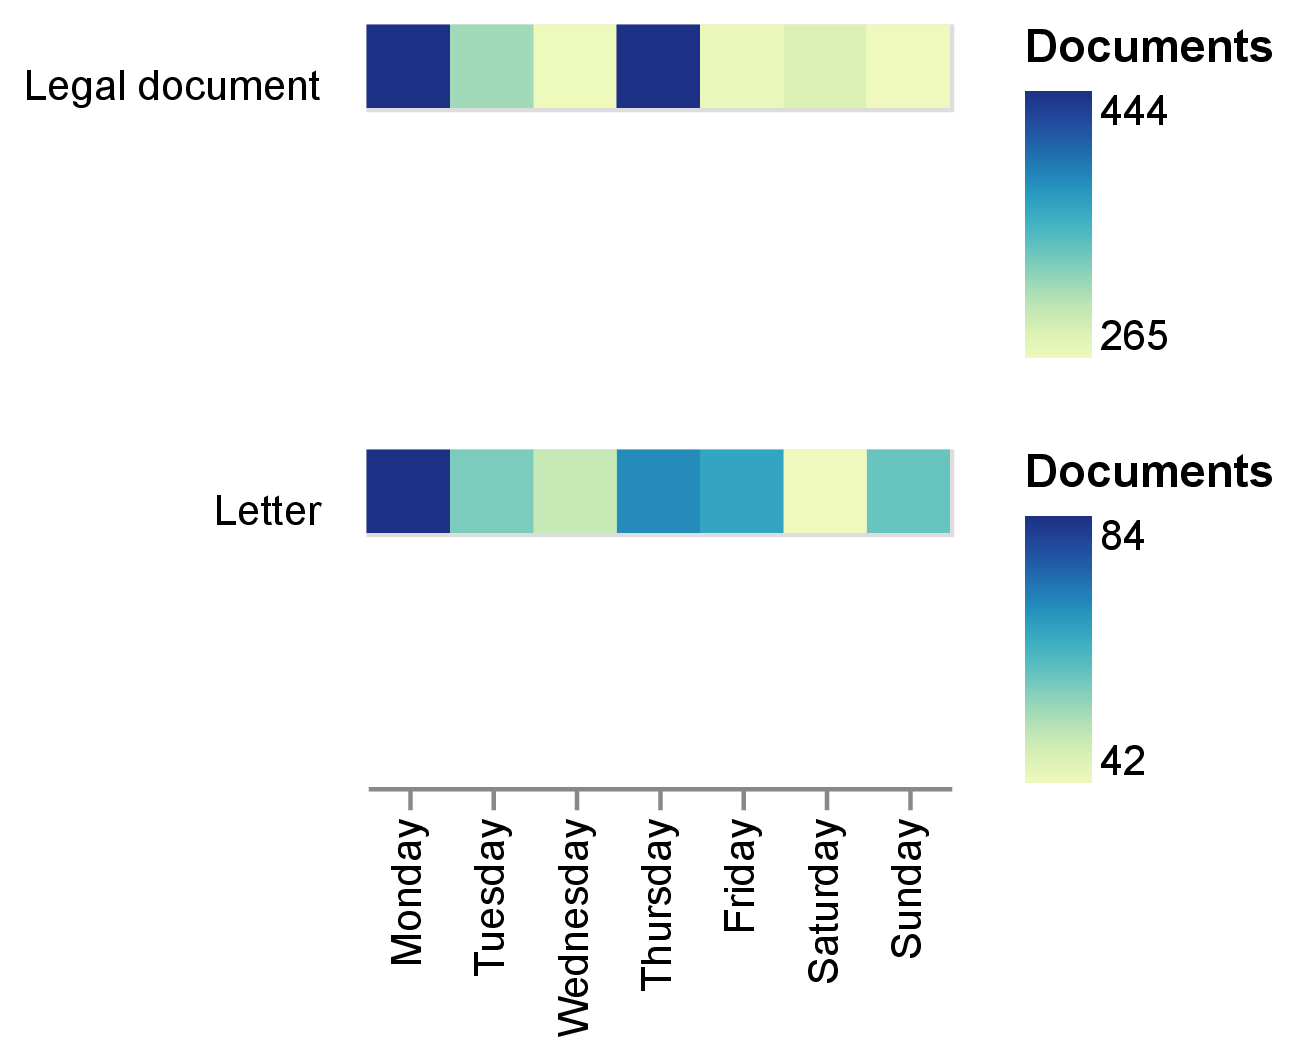
\includegraphics[width=0.4\linewidth]{figures/pgp_letters_legaldocs_weekday.png}
  \caption{Legal documents and letters frequency by weekday. }
  \label{fig:pgp-weekday-frequency}
\end{figure}


\subsection{Shakespeare and Company
Project}\label{shakespeare-and-company-project}

The \href{https://shakespeareandco.princeton.edu/}{\textit{Shakespeare and Company
Project}} is based on the materials from Sylvia Beach's famous
English-language lending library that operated in Paris in the 1920s
and 1930s. This project is one of the precursors that fed into the development of \texttt{undate}, with
an implementation to support incomplete dates written on handwritten cards \cite{kotin_shakespeare_2022, koeser_coding_2019}.

\begin{figure}[h]
  \centering
  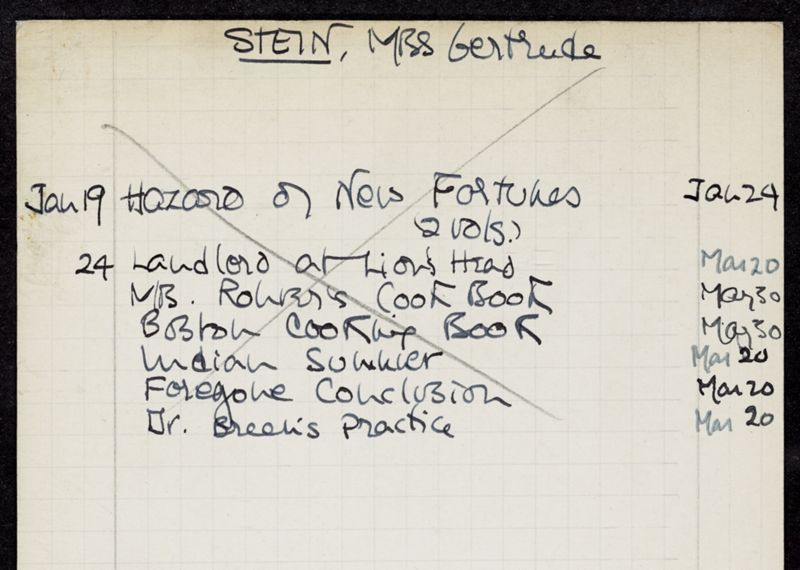
\includegraphics[width=0.7\linewidth]{figures/stein_lendingcard_unknownyear.jpg}
  \caption{Detail from Gertrude Stein's lending library card showing handwritten borrow events with no year. \cite{stein_beachpapers_pul, noauthor_gertrude_nodate} }
  \label{fig:stein-lending-card}
\end{figure}


\begin{table}[h]
  \centering 
  \begin{tabular}{lllrllrrl}
    \toprule
    Start Date & End Date & Duration & Title & Author \\ 
    \midrule
--01-19 & --01-24 & 5 & \textit{A Hazard of New Fortunes} & Howells, William Dean \\
--01-24 & --05-30 & 126 & \textit{Boston Cooking-School Cook Book} & Farmer, Fannie Merritt \\
--01-24 & --03-20 & 55 & \textit{The Landlord at Lion's Head} & Howells, William Dean \\
--01-24 & --05-30 & 126 & \textit{Mrs. Rorer's New Cook Book} & Rorer, Sarah Tyson \\
--01-24 & --03-20 & 55 & \textit{Indian Summer} & Howells, William Dean \\
--01-24 & --03-20 & 55 & \textit{A Foregone Conclusion} & Howells, William Dean \\
--01-24 & --03-20 & 55 & \textit{Dr. Breen's Practice} & Howells, William Dean \\
1920-04-29 & 1920-06-03 & 35 & \textit{The Letters of George Meredith} & Meredith, George \\
    \bottomrule
  \end{tabular}
  \caption{Sample borrowing activity for Gertrude Stein at the Shakespeare and Company lending library in Paris, including borrow events with unknown years but calculable durations.}
  \label{tab:stein-borrowing}
\end{table}


This project includes borrowing events with unknown years; with
\texttt{undate} we can calculate how long a book was borrowed even when
we don't know the exact year. We use Gertrude Stein as an example here, since she is a well known figure with documented borrowing activity without known years (Figure \ref{fig:stein-lending-card}), although she is far from the only one.\footnote{Stein is famous enough that these unknowns could perhaps be resolved through research; that is not the case for the lesser known members of this library.} Stein has 46 borrow events with calculable duration; of those 7, or 15\%, have no known year.  If we limit our analysis to borrow events with known years, we arrive at an average borrow length of 32 days and a maximum of 91 days. However, when we include events with unknown years we get an average of 38 and a maximum of 126 days. In the context of this project, we calculate the duration of borrow events with unknown years as the shortest possible duration between the start and end date; that is, the the dates are in the same year (or following year, when the end date is an earlier month than the start date). This is based on our assumption that the clerks working in the book shop would have noted the year if the book was out for a longer time period, as they did in other cases.

The full code used to calculate durations and plot them is available in Appendix \ref{appdx:shxco-duration-raincloud}.  Here we show a sample of the parsed borrow events (Table \ref{tab:stein-borrowing}) and a raincloud plot of Stein's borrowing (Figure \ref{fig:stein-borrow-raincloud}) to demonstrate the value of including partial information in our analysis. As you can see, leaving out partially known dates would greatly change the distribution. 


\begin{figure}[t!]
  \centering
  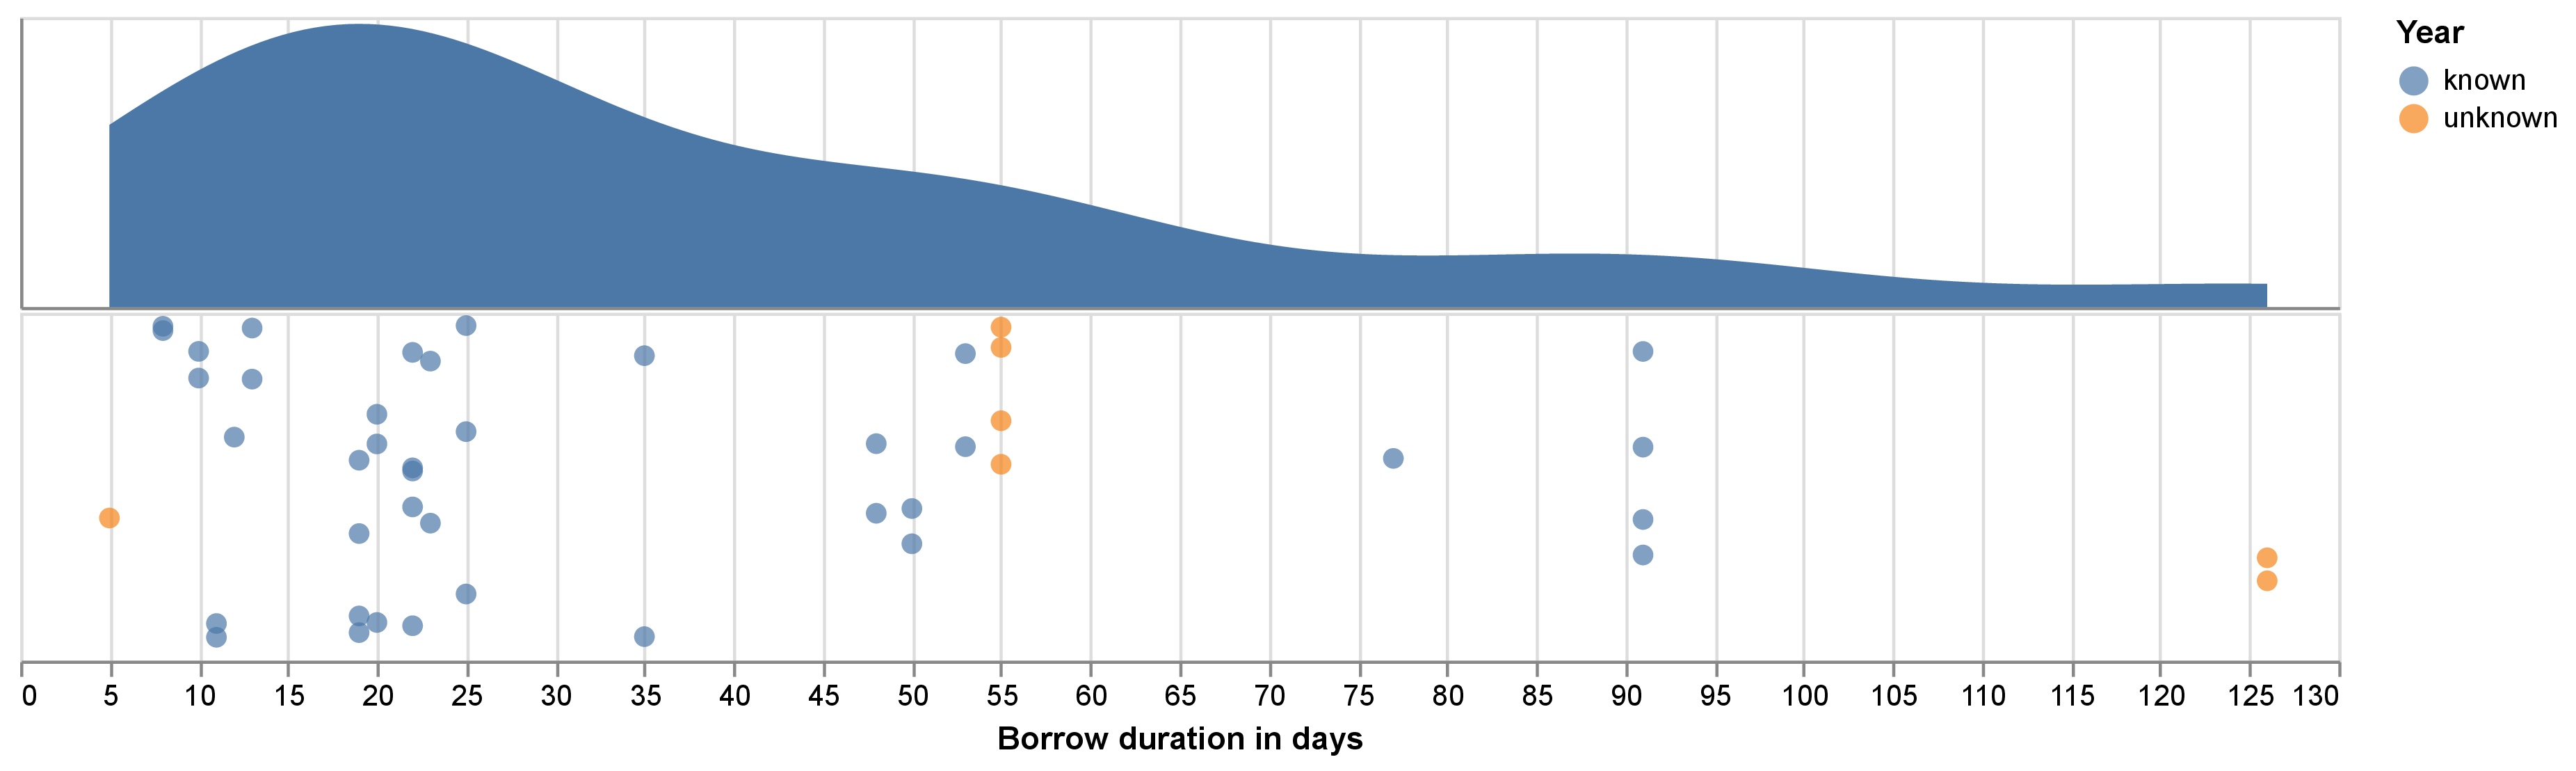
\includegraphics[width=\linewidth]{figures/shxco_stein_borrows.png}
  \caption{Raincloud plot showing how long Gertrude Stein typically kept the books
she borrowed.  Borrows with unknown years are highlighted in orange in the lower portion (the ``rain'') of the plot. }
  \label{fig:stein-borrow-raincloud}
\end{figure}

\section{Conclusion}

This paper provides a demonstration of some of the current functionality of the \texttt{undate} python library, although it is certainly not exhaustive. I have barely touched on intervals and some of the calculations and logic around uncertainty that are currently supported. This package is still in active development, with tremendous potential in multiple directions. I and my collaborators plan to continue adding support for more calendars and formats (e.g., RDF and CIDOC-CRM), and improve the support for ambiguity and granularity in parsing and date precisions.  Other avenues of interest are representing the temporal uncertainty in data visualizations based on \texttt{undate} parsing and analysis \cite{yau_visualizing_2018}, or making more use of labels for analysis. Development on \texttt{undate} input and use cases from the community to steer and prioritize the work, to ensure that work is interpretable and usable in the context of a specific project while still being general enough to be usable and accurate across disparate projects.  As \texttt{undate} matures, I hope to start seeing it used in more projects, and we would love to know if there is an interest or need in adapting it to other programming languages or extending it for specific ecosystems and frameworks.


\section*{Acknowledgements}
This work is supported by the Center for Digital Humanities at Princeton University.  Thanks to my reviewers, especially: David Ragnar Nelson, who caught and corrected several errors in the code examples introduced in the conversion from notebook to paper; and Julia Damerow, for suggestions to improve the flow.

% Print the biblography at the end. Keep this line after the main text of your paper, and before an appendix. 
\printbibliography

% You can include an appendix using the following command
\appendix

\section{Parsing PGP document dates in multiple calendars} \label{appdx:parse-pgp-dates}

Princeton Geniza Project data includes documents with original dates in multiple calendars.  \texttt{undate} does not yet provide an omnibus parser, so dates must be parsed according to their a known, supported calendar.  The dates in this dataset are complicated and messy, and include qualifiers and uncertainty not yet supported by \texttt{undat}e parsing. For demonstration purposes, this example code removes and ignores those complexities.

Adapted from an \href{https://github.com/dh-tech/undate-python/blob/main/examples/pgp_dates.ipynb}{example notebook} included in the \texttt{undate} software repository.

\begin{minted}{python}
import re

from lark.exceptions import UnexpectedEOF
from lark.visitors import VisitError
import polars as pl


# set this to True to see details about parsing
VERBOSE_PARSE_OUTPUT = False


def remove_ordinals(val):
    # utility method to turn ordinals into numerals
    # i.e., 1st, 2nd, 3rd -> 1, 2, 3
    return re.sub(r"(\d+)(st|nd|rd|th)", "\\1", val)


def parse_original_date(doc_date_original, doc_date_calendar):
    # Map PGP original calendar to undate calendar converter
    undate_calendar = None
    if doc_date_calendar == "Anno Mundi":
        undate_calendar = "Hebrew"
    elif doc_date_calendar == "Hijrī":
        undate_calendar = "Islamic"
    elif doc_date_calendar == "Seleucid":
        undate_calendar = "Seleucid"

    if undate_calendar:
        value = doc_date_original

        # some dates have unknown digits, e.g. 1[.] Kislev 48[..] or 152[.]
        # Replace with zeros for now, since the calendar parsers
        # doesn't yet support this syntax
        # (even though Undate supports unknown digits)
        if "[." in value:
            if VERBOSE_PARSE_OUTPUT:
                print(f"ignoring missing digits for now {value}")
            value = (
                value.replace("[.]", "0")
                .replace("[..]", "00")
                .replace("[...]", "000")
            )

        # some dates have inferred numbers, 
        # e.g. Friday, [25] Nisan [4810] or 8 Elul (4)811'
        # for now, we strip out brackets before parsing;
        # in future, we could indicate uncertainty based on these
        value = (
            value.replace("[", "")
            .replace("]", "")
            .replace("(", "")
            .replace(")", "")
        )

        # for now, remove modifiers not supported by the undate parser:
        #   Late Tevet 4903, Last decade of Kislev 5004, first third of ...
        modifiers = [
            "Late ",
            "(first|middle|last)( third|half|decade|tenth)? (of )?",
            "(Beginning|end) of ",
            "last day",
            "First 10 days",
            " of",
            "spring",
            "decade ",
            "night, ",
        ]
        for mod in modifiers:
            value = re.sub(mod, "", value, flags=re.I)

        # about 62 have ordinals; strip them out
        value = remove_ordinals(value)

        # parse the simplified, cleaned up date string 
        # with the specified calendar
        try:
            return Undate.parse(value, undate_calendar)
        except (VisitError, ValueError, UnexpectedEOF) as err:
            if VERBOSE_PARSE_OUTPUT:
                print(f"Parse error : {value} ({undate_calendar}): {err}")
            return None

# Use Polars to load data file into a DataFrame
# Filter to documents with standard dates
pgp_documents_df = pl.read_csv("pgp_documents.csv") \     
    .filter(
        pl.col("doc_date_standard").is_not_null()
    )
    
# Create a struct of original date and calendar,
# which we can pass to our parse method.
# If parsing succeeds, returns and Undate or UndateInterval
pgp_documents_df = pgp_documents_df.with_columns(
    undate_orig=pl.struct(
        "doc_date_original", "doc_date_calendar"
    ).map_elements(
        lambda row: parse_original_date(
            row["doc_date_original"], row["doc_date_calendar"]
        ),
        return_dtype=pl.datatypes.Object,
    )
)
days = [
    "Monday",
    "Tuesday",
    "Wednesday",
    "Thursday",
    "Friday",
    "Saturday",
    "Sunday",
]

# filter to records that were successfully parsed; 
# determine weekday for use with day-level precision dates

pgp_documents_df = (
    pgp_documents_df.filter(pl.col("undate_orig").is_not_null())
    .with_columns(
        pl.col("type").fill_null("Unknown"),  # set null type to unknown
        orig_date_precision=pl.col("undate_orig").map_elements(
            lambda x: str(x.precision).lower(),
            return_dtype=pl.datatypes.String,
        ),
        undate_weekday=pl.col("undate_orig").map_elements(
            lambda x: x.earliest.weekday, return_dtype=pl.datatypes.Int32
        ),
    )
    .with_columns(
        undate_weekday_name=pl.col("undate_weekday").map_elements(
            lambda x: days[x], return_dtype=pl.datatypes.String
        )
    )
)

# filter to relevant fields and display the first ten rows
pgp_documents_df.select(
    "pgpid",
    "type",
    "doc_date_original",
    "doc_date_calendar",
    "doc_date_standard",
    "undate_orig",
    "orig_date_precision",
    "undate_weekday_name",
).head(10)    
\end{minted}

\section{Determine and plot durations for Shakespeare and Company Project borrowing}\label{appdx:shxco-duration-raincloud}

This project includes borrowing events with unknown years; with \texttt{undate} we can calculate how long a book was borrowed even when we don't know the year. 

First we define a couple of methods that we'll use with the data:
\begin{itemize}
    \item \texttt{undate\_duration} to parse the dates and calculate duration in days
    \item \texttt{known\_year} to provide an indicator for whether the year was known, which we'll use when plotting the data
\end{itemize}

We load the full events data from the Shakespeare and Company published datasets \cite{koeser_shakespeare_2025} and filter it to borrow events for Gertrude Stein based on \texttt{event\_type} and \texttt{member\_ids}.  Then we use the custom methods defined first to calculate borrow durations and add a variable indicating whether the year is known.

Finally, we define and use a method to generate a raincloud plot, showing the distribution of borrow durations in two different ways, and color the rain drops in the lower portion of the plot to highlight the durations based on borrow events with unknown years. (The raincloud plot is adapted from prior work in \cite{koeser_missing_2024}.)

\begin{minted}{python}
import altair as alt

from undate import UndateInterval
from undate.date import ONE_DAY, UnInt
from undate.converters.iso8601 import ISO8601DateFormat


def undate_duration(start_date, end_date):
    isoformat = ISO8601DateFormat()

    unstart = isoformat.parse(start_date)
    unend = isoformat.parse(end_date)
    interval = UndateInterval(earliest=unstart, latest=unend)

    # borrow durations in Shakespeare and Company Project were defined as
    # not including both ends (or half of the day on both ends);
    # to reconcile differences between duration logic with undate, 
    # which includes both endpoints, we subtract one day
    return (interval.duration() - ONE_DAY).days


def known_year(date):
    return "known" if ISO8601DateFormat().parse(date).known_year else "unknown"


stein_borrow_events_df = (
    pl.read_csv("SCoData_events_v2.0_2025.csv", infer_schema_length=10000)
    .filter(
        pl.col("member_ids").eq("stein-gertrude"),
        pl.col("event_type").eq("Borrow"),
        # for simplicity, we're going to limit to events that Project
        # provides a borrow duration for; this indicates
        # the duration is calculable (i.e., start and end dates known)
        pl.col("borrow_duration_days").is_not_null(),
    )
    .select(
        "event_type",
        "start_date",
        "end_date",
        "borrow_duration_days",
        "item_title",
        "item_authors",
        "item_year",
    )
)

# calculate durations; returns a dataframe with one column
duration_df = stein_borrow_events_df.select("start_date", "end_date").map_rows(
    lambda x: undate_duration(x[0], x[1]), return_dtype=pl.datatypes.Int32
)

# add fields to the main dataframe for duration and whether year is known
stein_borrow_events_df = stein_borrow_events_df.with_columns(
    undate_duration=duration_df["map"],
    known_year=stein_borrow_events_df["start_date"].map_elements(
        known_year, return_dtype=pl.datatypes.String
    ),
)


def raincloud_plot(dataset, fieldname, field_label, color_opts=None):
    """Create a raincloud plot for the density of the specified field
    in the given dataset. Takes an optional tooltip for the strip plot.
    Returns an altair chart."""

    # create a density area plot of specified fieldname

    duration_density = (
        alt.Chart(dataset)
        .transform_density(
            fieldname,
            as_=[fieldname, "density"],
        )
        .mark_area(orient="vertical")
        .encode(
            x=alt.X(
                fieldname, title=None, axis=alt.X(labels=False, ticks=False)
            ),
            y=alt.Y(
                "density:Q",
                # suppress labels and ticks because we're going to combine this
                title=None,
                axis=alt.Axis(
                    labels=False, values=[0], grid=False, ticks=False
                ),
            ),
        )
        .properties(height=100, width=800)
    )

    # Now create jitter plot of the same field
    # jittering / stripplot adapted from https://stackoverflow.com/a/71902446/9706217

    chart_color_opts = {}
    if color_opts is not None:
        chart_color_opts = {"color": color_opts}

    stripplot = (
        alt.Chart(dataset)
        .mark_circle(size=50)
        .encode(
            x=alt.X(
                fieldname,
                title=field_label,
                axis=alt.Axis(labels=True),
            ),
            y=alt.Y("jitter:Q", title=None, axis=None),
            **chart_color_opts,
            # color=alt.Color(color_by),  # .scale(**color_scale),
        )
        .transform_calculate(jitter="(random() / 200) - 0.0052")
        .properties(
            height=120,
            width=800,
        )
    )

    # use vertical concat to combine the two plots together
    raincloud_plot = alt.vconcat(duration_density, stripplot).configure_concat(
        spacing=0
    )
    return raincloud_plot


stein_borrows_plot = raincloud_plot(
    stein_borrow_events_df,
    "undate_duration",
    "Borrow duration in days",
    alt.Color("known_year", title="Year"),
)

\end{minted}



\end{document}
 
\section{First Appendix Section} \label{appdx:first}

Appendix sections should be ordered by letters rather than numbers, and their contents do not count towards the paper's length limit. Appendix sections may also contain additional tables and figures.  

\end{document}
